% Drawing 69/01-4 -- folder 69, batch 01, archive page 6 (PDF page 7).
% Transcription: en haut à gauche, une rangée de petits schémas : des segments aux extrémités marquées $x\ x'$, $y\ y'$, $\xi\ \xi'$, $\eta\ \eta'$, $s\ s'$, $t\ t'$, surmontés d'arcs en chevrons qui relient les segments, et sous eux des colonnes $\binom{s}{t}$, $\binom{s'}{t'}$, $\binom{s}{t'}$, $\binom{s'}{t}$, $\binom{x}{y}$, $\binom{x'}{y'}$, $\binom{x}{y'}$, $\binom{x'}{y}$ ; un trait vertical sépare les deux premiers groupes, et le dernier groupe (avec $u'$, $v'$) est couvert de hachures
% Kind: row of small schemas (segments, chevrons, columns). Method 2 (schematic redraw from the facsimile). Status: partial.
% Notes: Row of small segments with marked ends: x x', y y' (dots), xi xi', eta eta', s s' and t t' (thick), with chevron arcs over the s/t segments and over the last, hatched group (whose right end carries u'); under them four groups of columns s/t, s/t, x/y, x/y. A vertical stroke separates the first two groups. The column contents are written as the transcription gives them (s t, s' t', s t', s' t; x y, ...), the small letters on the page being only partly legible; the last group is heavily overwritten (hatching drawn as a hatched band).
% Coordinates: 1 unit = 1 mm = 1/100 of the crop width (bbox in page fractions: [0.06, 0.1, 0.62, 0.24]).
% Redrawn by Claude (claude-opus-5-5), issue #73, 2026-11-07; not checked by a human; not compiled (no TeX in the session).
% Rights: reproduces part of the work -- behind RENDER_TRANSCRIPTS, never published by itself.
\documentclass[tikz,border=3pt]{standalone}
\usepackage{amsmath,amssymb}
\usetikzlibrary{patterns,arrows.meta}
\tikzset{pencil/.style={black!45}, struck/.style={black!35}, mark/.style={circle,draw,inner sep=1.3pt}, pt/.style={circle,fill,inner sep=0.9pt}, opt/.style={circle,draw,fill=white,inner sep=1.1pt}}
\begin{document}
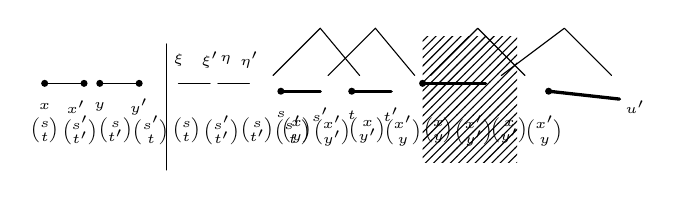
\begin{tikzpicture}[x=1mm,y=1mm,line cap=round,line join=round,font=\scriptsize]
\draw (12,-20) -- (17,-20);
\node[pt] at (12,-20) {};
\node[pt] at (17,-20) {};
\draw (19,-20) -- (24,-20);
\node[pt] at (19,-20) {};
\node[pt] at (24,-20) {};
\node[inner sep=1pt] at (12,-23) {\tiny $x$};
\node[inner sep=1pt] at (16,-23) {\tiny $x'$};
\node[inner sep=1pt] at (19,-23) {\tiny $y$};
\node[inner sep=1pt] at (24,-23) {\tiny $y'$};
\draw (29,-20) -- (33,-20);
\draw (34,-20) -- (38,-20);
\node[inner sep=1pt] at (29,-17) {\tiny $\xi$};
\node[inner sep=1pt] at (33,-17) {\tiny $\xi'$};
\node[inner sep=1pt] at (35,-17) {\tiny $\eta$};
\node[inner sep=1pt] at (38,-17) {\tiny $\eta'$};
\draw (27.5,-15) -- (27.5,-31);
\draw[very thick] (42,-21) -- (47,-21);
\draw[very thick] (51,-21) -- (56,-21);
\node[pt] at (42,-21) {};
\node[pt] at (51,-21) {};
\node[inner sep=1pt] at (42,-24) {\tiny $s$};
\node[inner sep=1pt] at (47,-24) {\tiny $s'$};
\node[inner sep=1pt] at (51,-24) {\tiny $t$};
\node[inner sep=1pt] at (56,-24) {\tiny $t'$};
\draw (41,-19) -- (47,-13) -- (52,-19);
\draw (48,-19) -- (54,-13) -- (59,-19);
\draw[very thick] (60,-20) -- (68,-20);
\node[pt] at (60,-20) {};
\draw (61,-19) -- (67,-13) -- (73,-19);
\draw (70,-19) -- (78,-13) -- (84,-19);
\draw[very thick] (76,-21) -- (85,-22);
\node[pt] at (76,-21) {};
\node[inner sep=1pt] at (87,-23) {\tiny $u'$};
\fill[pattern=north east lines] (60,-14) -- (72,-14) -- (72,-30) -- (60,-30) -- cycle;
\node[inner sep=1pt] at (12,-26) {\tiny $\binom{s}{t}$};
\node[inner sep=1pt] at (16.5,-26) {\tiny $\binom{s'}{t'}$};
\node[inner sep=1pt] at (21,-26) {\tiny $\binom{s}{t'}$};
\node[inner sep=1pt] at (25.5,-26) {\tiny $\binom{s'}{t}$};
\node[inner sep=1pt] at (30,-26) {\tiny $\binom{s}{t}$};
\node[inner sep=1pt] at (34.5,-26) {\tiny $\binom{s'}{t'}$};
\node[inner sep=1pt] at (39,-26) {\tiny $\binom{s}{t'}$};
\node[inner sep=1pt] at (43.5,-26) {\tiny $\binom{s'}{t}$};
\node[inner sep=1pt] at (44,-26) {\tiny $\binom{x}{y}$};
\node[inner sep=1pt] at (48.5,-26) {\tiny $\binom{x'}{y'}$};
\node[inner sep=1pt] at (53,-26) {\tiny $\binom{x}{y'}$};
\node[inner sep=1pt] at (57.5,-26) {\tiny $\binom{x'}{y}$};
\node[inner sep=1pt] at (62,-26) {\tiny $\binom{x}{y}$};
\node[inner sep=1pt] at (66.5,-26) {\tiny $\binom{x'}{y'}$};
\node[inner sep=1pt] at (71,-26) {\tiny $\binom{x}{y'}$};
\node[inner sep=1pt] at (75.5,-26) {\tiny $\binom{x'}{y}$};
\end{tikzpicture}
\end{document}
